\documentclass{standalone}
\usepackage{tikz}
\begin{document}
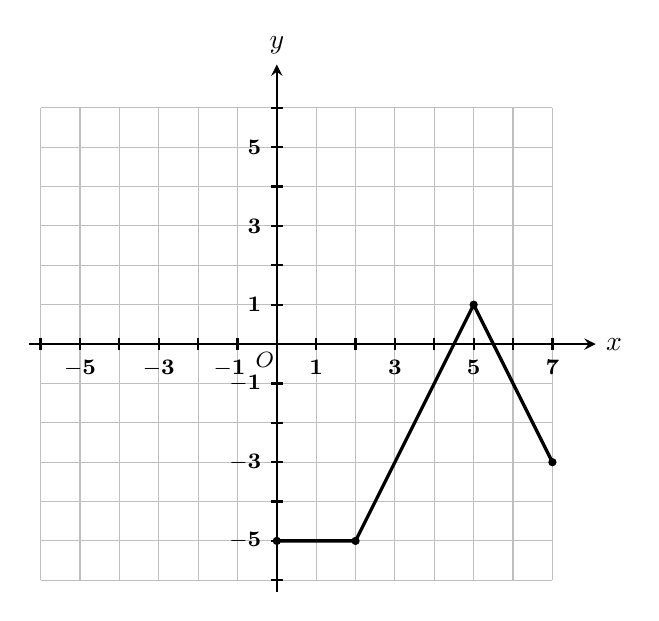
\begin{tikzpicture}[color=black, >=stealth, scale=0.5]
  % Grid: x from -6 to 7, y from -6 to 6
  \draw[gray!50, thin] (-6,-6) grid (7,6);
  % Axes (arrows only on the positive ends, as in the original)
  \draw[->, thick] (-6.3,0) -- (8.1,0) node[right] {$x$};
  \draw[->, thick] (0,-6.3) -- (0,7.1) node[above] {$y$};
  % Tick marks at every integer
  \foreach \x in {-6,...,7} \draw[thick] (\x,0.15) -- (\x,-0.15);
  \foreach \y in {-6,...,6} \draw[thick] (0.15,\y) -- (-0.15,\y);
  % Tick labels at odd values only
  \foreach \x in {-5,-3,1,3,5,7}
    \node[font=\footnotesize\bfseries, below] at (\x,-0.15) {$\mathbf{\x}$};
  % -1 nudged left so it clears the O label, as in the original
  \node[font=\footnotesize\bfseries, below] at (-1.2,-0.15) {$\mathbf{-1}$};
  \foreach \y in {-5,-3,-1,1,3,5}
    \node[font=\footnotesize\bfseries, left] at (-0.15,\y) {$\mathbf{\y}$};
  \node[font=\footnotesize] at (-0.3,-0.4) {$O$};
  % Piecewise-linear graph: (0,-5) -- (2,-5) -- (5,1) -- (7,-3)
  \draw[line width=1.2pt] (0,-5) -- (2,-5) -- (5,1) -- (7,-3);
  % Filled endpoints and corners
  \foreach \p in {(0,-5),(2,-5),(5,1),(7,-3)} \fill[black] \p circle (3pt);
\end{tikzpicture}
\end{document}
